\documentclass{article}
\usepackage{ctex}
\title{编译原理 作业1}
\author{} 
\date{}
\usepackage[a4paper,left=10mm,right=10mm,top=15mm,bottom=15mm]{geometry} 
\usepackage{graphicx} 
\begin{document}
\section*{2.6}
\noindent 
\textbf{(1)}由0~9的数字形成的非空串,$L(G_6)=\{a^n|a\in\{0,1,\dots,9\}\}$\\
\textbf{(2)}0127的最左推导:$N\Rightarrow ND\Rightarrow NDD\Rightarrow NDDD\Rightarrow DDDD\Rightarrow 0DDD\Rightarrow
01DD\Rightarrow 012D\Rightarrow 0127$.\\
0127的最右推导:$N\Rightarrow ND \Rightarrow N7 \Rightarrow ND7 \Rightarrow N27 \Rightarrow ND27 \Rightarrow N127
\Rightarrow D127 \Rightarrow 0127$.\\
34的最左推导:$N\Rightarrow ND \Rightarrow DD\Rightarrow 3D \Rightarrow 34$.\\
34的最右推导:$N\Rightarrow ND \Rightarrow N4 \Rightarrow D4 \Rightarrow 34$.\\
568的最左推导:$N\Rightarrow ND\Rightarrow NDD\Rightarrow DDD\Rightarrow 5DD\Rightarrow 56D\Rightarrow 568$.\\
568的最右推导:$N\Rightarrow ND\Rightarrow N8\Rightarrow ND8\Rightarrow N68 \Rightarrow D68\Rightarrow 568$.
\section*{2.7}
\noindent 
首先得到从正奇数生成所有奇数的文法$O\rightarrow O_{+}|-O_{+}$.\\
所有一位非零偶数与一位非零奇数的文法为$E_0\rightarrow 2|4|6|8,O_0\rightarrow 1|3|5|7|9$,
则一个正奇数的头部文法为$H\rightarrow E_0|O_0|\epsilon$.\\
任意一位数字的文法为$A_0\rightarrow 0|E_0|O_0$,
则一个正奇数的中部文法为$M\rightarrow A_0|MA_0|\epsilon$.\\
则有正奇数文法$O_{+}\rightarrow HMO_0$.
\section*{2.8}
\noindent 
\textbf{(1)}$i+i*i$的最左推导:$E\Rightarrow E+T\Rightarrow T+T\Rightarrow F+T\Rightarrow i+T\Rightarrow i+T*F\Rightarrow i+F*F\Rightarrow i+i*F\Rightarrow i+i*i$\\
$i+i*i$的最右推导:$E\Rightarrow E+T\Rightarrow E+T*F\Rightarrow E+T*i\Rightarrow E+F*i\Rightarrow E+i*i\Rightarrow T+i*i\Rightarrow F+i*i\Rightarrow i+i*i$\\
$i*(i+i)$的最左推导:$E\Rightarrow T \Rightarrow T*F\Rightarrow F*F\Rightarrow i*F\Rightarrow i*(E)\Rightarrow i*(E+T)\Rightarrow i*(T+T)\Rightarrow i*(F+T)\Rightarrow i*(i+T)\Rightarrow i*(i+F)\Rightarrow i*(i+i)$\\
$i*(i+i)$的最右推导:$E\rightarrow T\rightarrow T*F\rightarrow T*(E)\rightarrow T*(E+T)\rightarrow T*(E+F)\rightarrow T*(E+i)\rightarrow T*(T+i)\rightarrow T*(F+i)\rightarrow T*(i+i)\rightarrow F*(i+i)\rightarrow i*(i+i)$\\
\textbf{(2)}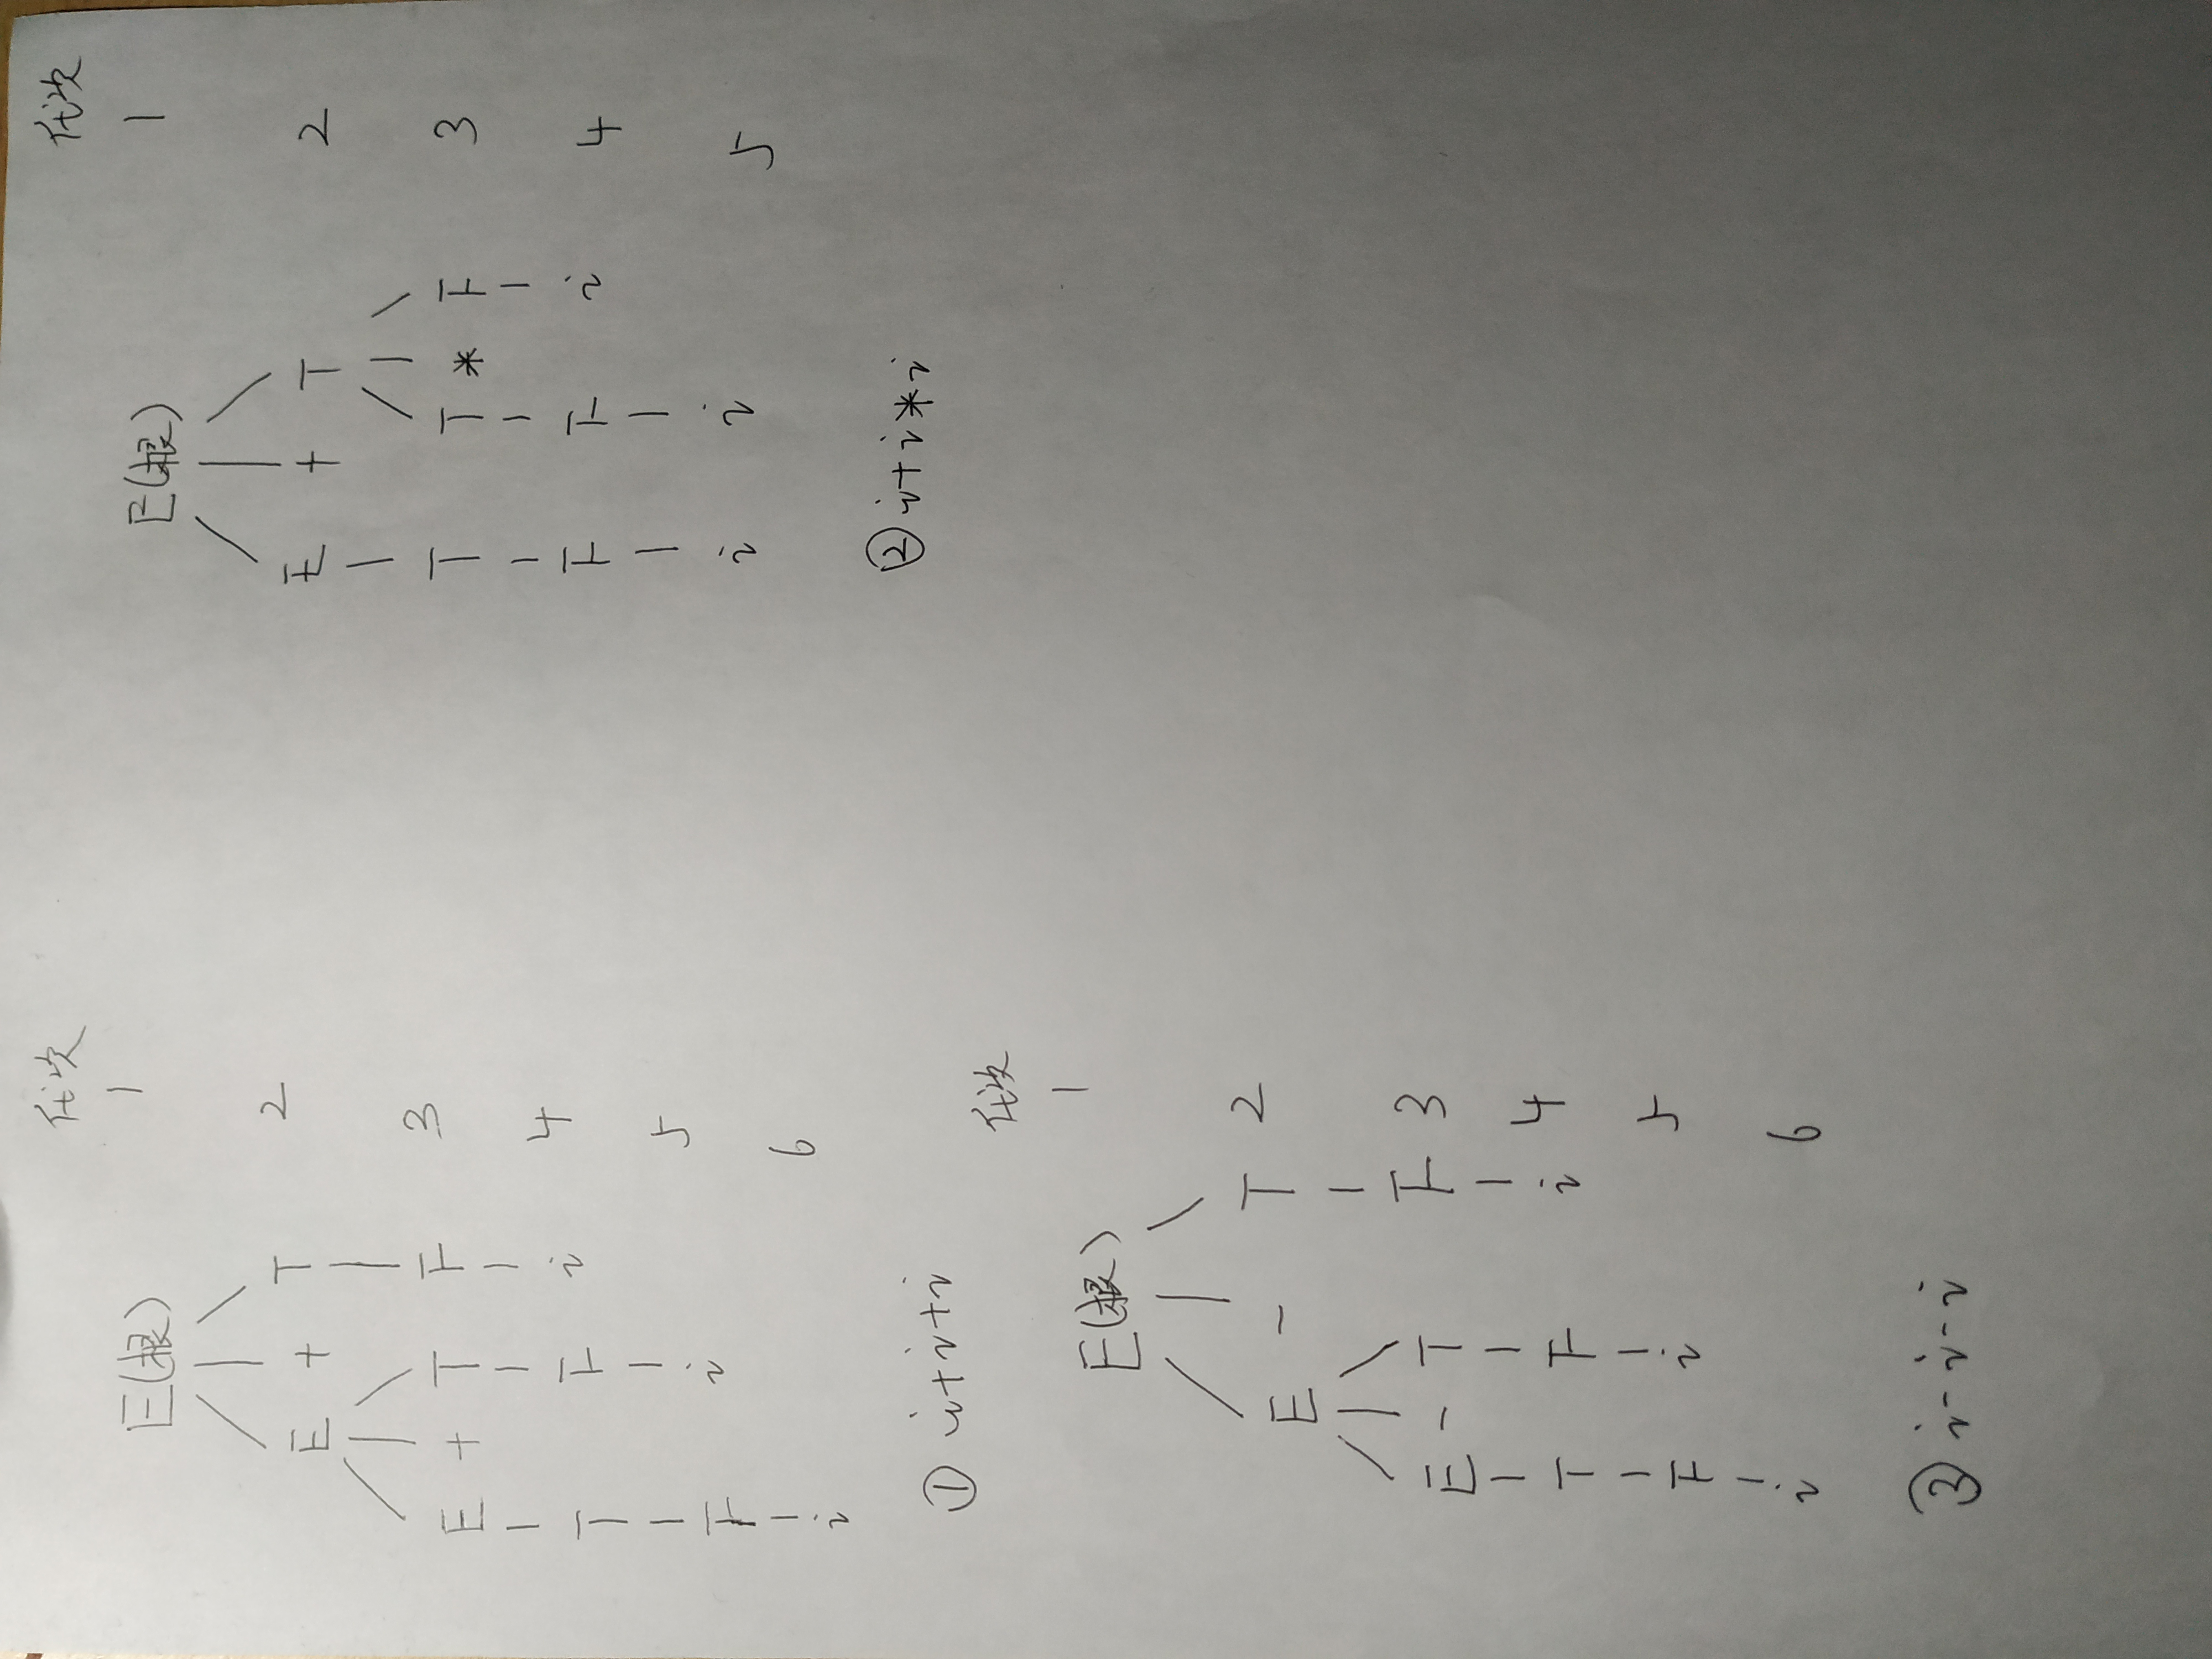
\includegraphics[height=8cm,angle=270]{1_1.jpg}
\section*{2.9}
\noindent 
对于$iiiei$,有如下两种不同的最右推导:
\begin{itemize}
    \item [-] $S\Rightarrow iS\Rightarrow iiSeS\Rightarrow iiSei\Rightarrow iiiei$
    \item [-] $S\Rightarrow iSeS\Rightarrow iSei\Rightarrow iiSei\Rightarrow iiiei$
\end{itemize}
因此该文法是二义的.
\section*{2.10}
\noindent 
对于本文法,$()()()$可产生两种不同的最左推导:
\begin{itemize}
    \item [-] $S\Rightarrow SS\Rightarrow SSS\Rightarrow ()SS\Rightarrow ()()S\Rightarrow ()()()$
    \item [-] $S\Rightarrow SS\Rightarrow ()S\Rightarrow ()SS\Rightarrow ()()S\Rightarrow ()()()$
\end{itemize}
在$S$产生$SS$的过程中,如果通过调整文法的方式保证其中一个$S$被求值,这样就可以确定结合的顺序,从而避免二义性,故调整文法如下:\\
$S\rightarrow S(T)|(S)|()\\
T\rightarrow S|\epsilon$
\section*{2.11}
\noindent 
\textbf{(1)}$G_1\rightarrow ab|aG_1b,C_*\rightarrow cC_*|\epsilon,$\\
则$L_1\rightarrow G_1C_*$\\
\textbf{(2)}$G_2\rightarrow bc|bG_2c,A_*\rightarrow aA_*|\epsilon,$\\
则$L_2\rightarrow A_*G_2$\\
\textbf{(3)}$G_3\rightarrow aG_3b|\epsilon,$则$L_3\rightarrow G_3G_3$\\
\textbf{(4)}$G_4\rightarrow 0G_41|\epsilon,$则$L_4\rightarrow G_4|1G_40$

\end{document}
